% Some commands used in this file
%\newcommand{\package}{\emph}

\chapter{Introduction}
\label{chap:intro}

\section{Mobile Robotics}
\label{sec:mobile robotics}

Mobile robotics has shown significant developments in the last years resulting in growing areas of applications from Mars exploration (Figure ~\ref{fig:curiosity}) to house cleaning. Within this growth, mobile robots varied in the ways of their movement, in their target environments and applications. Hence, they have spread into more branches which include quite new research areas. A rough classification of mobile robots can be made as follows;

\begin{description}
	\item[Type of structure] 
\end{description}
\begin{itemize}
	\item Legged robots 
	\item Tracks
  \item Wheeled robots 
\end{itemize}
\begin{description}
	\item[Operating environment] 
\end{description}
\begin{itemize}
	\item Indoor robots 	
	\item Space robots 
  \item Land robots (Unmanned Ground Vehicles - UGVs)
	\item Underwater robots (Autonomous Underwater Vehicles - AUVs)
	\item Aerial robots (Unmanned Aerial Vehicles - UAVs) 
	\item Polar robots
\end{itemize}
\begin{description}
	\item[Application area] 
\end{description}
\begin{itemize}
	\item Service robots
  \item Cleaning robots
  \item Field robots 
	\item Social robots
	\item Material handling robots
\end{itemize}

\begin{figure}
	\centering
	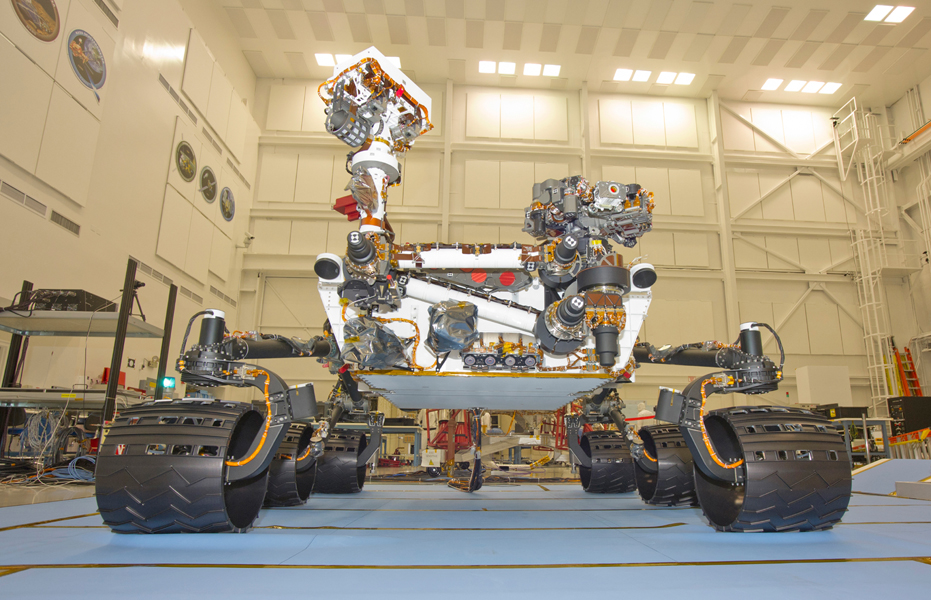
\includegraphics[scale=1.4]{images/img1-mars-rover}
	\caption{Front view of Mars Curiosity rover, Courtesy NASA/JPL-Caltech \cite{curiosity}}
	\label{fig:curiosity}
\end{figure}

The classification can be varied with new application areas and technologies. Although the specific applications are developed depending on the type and target task of the mobile robots, they share several cases to be handled such as sensor reading, tele-operation, to estimate the position and orientation, navigation and so on. These cases form the basics of a mobile robot application development. 

\section{Goal}
\label{sec:goal}
In this project, it is aimed to develop base applications using Robot Operating System (ROS) framework for the mobile robots of the type Autonomous Guided Vehicle (AGV) at Istanbul Technical University Robotics Laboratory named ITU-AGVs. The goal covers developing embedded software to be able to communicate with the microcontroller and developing on ROS framework for base tasks including simulation, sensor integration and reading, tele-operation, estimation of position and orientation, data collection and offline map building. It is aimed to provide these operations so that, they can be used as a basis –which ITU-AGVs lack– for developing specific applications. 


\section{Organization}
\label{sec:organization}
It is necessary to provide a background information in order to emphasize the project work. Hence in Chapter 2, information regarding Autonomous Guided Vehicles together with the details of ITU-AGVs are given and the kinematic model is derived. In Chapter 3, basics of Robot Operating System are provided with a brief review. Afterwards, all the work regarding the application development process is told in detailed in Chapter 4 and its subsections. Then, the overall outcomes, conclusions and possible future work are given in Chapter 5. 